%----------------------------------------------------------------------------------------
%	PACKAGES AND THEMES
%----------------------------------------------------------------------------------------

\documentclass{beamer}


\setbeamercovered{transparent}

\usetheme{Madrid}

\usepackage{graphicx} % Allows including images
\usepackage{booktabs} % Allows the use of \toprule, \midrule and \bottomrule in tables
\usepackage{url}
\usepackage[czech]{babel}
\usepackage[utf8]{inputenc}
\usepackage[T1]{fontenc}
\usepackage{amsfonts, amssymb, amsmath, amsthm}
\usepackage{tikz}
\usepackage{multirow}
\usepackage{listings}
\usepackage{mathtools}
\usetikzlibrary{calc}

\makeatletter
\begingroup
\toks0=\expandafter{\@cline{#1}-{#2}\@nil}
\@ifpackageloaded{booktabs}{%
  \toks2=\expandafter{\@@@cmidrule[{#1}-{#2}]{#3}{#4}}%
}{}
\catcode`-=\active
\edef\x{\gdef\unexpanded{\@cline#1-#2\@nil}{\the\toks0}}\x
\@ifpackageloaded{booktabs}{%
  \edef\x{\gdef\unexpanded{\@@@cmidrule[#1-#2]#3#4}{\the\toks2}}\x
}{}
\endgroup
\makeatother

%----------------------------------------------------------------------------------------
%	TITLE PAGE
%----------------------------------------------------------------------------------------

\title[Přerozdělení oblastí v grafu]{Přerozdělení oblastí v grafu založené na technikách rozkladu řídkých matic}
\subtitle{Graph repartitioning based on sparse matrix factorization techniques}

\author{Bc. Vladislav Matúš} % Your name
\institute[FJFI ČVUT]
{
  České vysoké učení technické v Praze \\
  Fakulta jaderná a fyzikálně inženýrská  \\ % Your institution for the title page
\medskip
Obor Matematická informatika
}
\date{}


\uselanguage{Czech}
\languagepath{Czech}

\deftranslation[to=Czech]{Definition}{Definice}


\begin{document}


\begin{frame}
	\titlepage
\end{frame}

%----------------------------------------------------------------------------------------
%	OVERVIEW
%----------------------------------------------------------------------------------------

\begin{frame}
	\only
	\frametitle{Obsah}
	\tableofcontents[]
\end{frame}

%----------------------------------------------------------------------------------------
	\section{Motivace}
%----------------------------------------------------------------------------------------

\begin{frame}
  \frametitle{Choleského rozklad matice}	
  \begin{itemize}
    \item Úplný rozklad matice
    \medskip
    \item Symetrická eliminace $A=LDL^T$
    \medskip
    \item \textbf{Choleského rozklad} $A=LL^T$
    \medskip
    \item Motivace:
      \begin{align*}
      &A\vec{x} = \vec{b}, \ A=LL^T    \\
      &L^T\vec{x}=\vec{y}, \ L\vec{y}=\vec{b}
      \end{align*}
  \end{itemize}
\end{frame}

\begin{frame}
  \frametitle{Dělení grafu jako nástroj pro manipulaci s maticemi}
  \begin{itemize}
    \item Dělení grafu $G=(V,E)$ 
    \medskip
    \begin{itemize}
      \item Rozklad množiny $V$ s počtem vrcholů $n$ na podmnožiny $V_1,...V_k$.
      \medskip
      \item Základní kritéria:
      \begin{itemize}
        \item$|V_i| = n/k$
        \item Minimalizace velikosti separátoru
      \end{itemize}
    \end{itemize}
    \medskip
    \item Vztah grafu a matice:
      \begin{figure}
        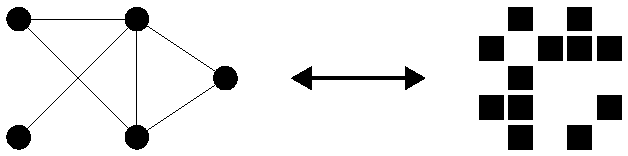
\includegraphics[width=200px]{images/matgr.pdf}
      \end{figure}
    \medskip
    \item Dělení pomocí vrcholového separátoru
  \end{itemize}
\end{frame}

\begin{frame}
	\frametitle{Cíle}
  \begin{enumerate}
    \item Analyzovat dělení grafu jako nástroj pro paralelizaci Choleského rozkladu matice
    \medskip
    \item Minimalizovat počet nenulových prvků v Choleského faktoru na oblastech pomocí číslování
    \medskip
    \item Prozkoumat vliv aposteriorního přerozdělení grafu na vyváženost počtu nenulových prvků ve faktorech
  \end{enumerate}
\end{frame}

%----------------------------------------------------------------------------------------
	\section{Techniky}
%----------------------------------------------------------------------------------------
\begin{frame}
  \frametitle{Analýza vhodnosti daného rozdělení grafu}
  \begin{itemize}
    \item Základní kritéria nepokrývají vyváženost Choleského rozkladu
    \medskip
    \item Eliminační stromy:
    \[\texttt{PARENT}[j] := \min \left\{ i > j \ | \ [L]_{i,j} \neq 0\right\}
    \]
  \end{itemize}
\end{frame}


\begin{frame}
  \frametitle{Číslování vrcholů grafu}
  \begin{itemize}
    \item Číslování vrcholů podle vzdálenosti
    \medskip
    \item Metoda minimálního stupně
    \medskip
    \item Smíšené číslování:
    \medskip
    \begin{itemize}
      \item Současné použití předchozích kritérií
      \medskip
      \item Konvexní kombinace: \ $\varphi(v) + (1-\alpha)\psi(v)$
    \end{itemize}
  \end{itemize}
\end{frame}

\begin{frame}
  \frametitle{Přesun separátoru}
  \begin{itemize}
    \item Konstrukce nového separátoru:
      \medskip
      \begin{enumerate}
          \item Přidáme $(G_{max} \cap\mathrm{adj}(S))$
          \medskip
          \item Odebereme nadbytečné vrcholy
        \end{enumerate}
      \medskip
    \item Pro nevyvážená rozdělení
    \medskip
    \item Reálné matice $\Rightarrow$ malá degradace separátoru
  \end{itemize}
\end{frame} 

%----------------------------------------------------------------------------------------
	\section{Výsledky}
%----------------------------------------------------------------------------------------

\begin{frame}
    \frametitle{Vliv číslování na počet nenulových prvků v Choleského faktorech}

    \begin{table}[ht]
      \tiny
      \centering
      \renewcommand{\arraystretch}{1.15}
    \begin{tabular}{|l|c|c|c|r|r|r|}
      \hline
      \multicolumn{1}{|c|}{Matice} & \multicolumn{1}{|c|}{$|S|$}    &\multicolumn{1}{|c|}{$|V_1|$} &\multicolumn{1}{|c|}{$|V_2|$} & \multicolumn{1}{|c|}{\texttt{-ot}} & \multicolumn{2}{c|}{Počty nenul} \\
      \hline
      \multirow{4}{*}{P100}
      &	\multirow{4}{*}{100}	&	\multirow{4}{*}{4950}	&	\multirow{4}{*}{4950}	&\texttt{-}&	241249	&	240331	\\
      &	&	&	&\texttt{DIST}&	461142	&	465406	\\
      &	&	&	&\texttt{MD}&	89757	&	91915	\\
      &	&	&	&\texttt{MIX}&	91152	&	89384	\\
      \hline
      \multirow{4}{*}{1138\_bus.rb}
      &	\multirow{4}{*}{5}	&	\multirow{4}{*}{653}	&	\multirow{4}{*}{480}	&\texttt{-}    &	14529	&	7876	\\
      & & & &\texttt{DIST} &	2361	&	1251	\\
      & & & &\texttt{MD}   &	1215	&	783	\\
      & & & &\texttt{MIX}  &	1227	&	782	\\
      \hline
      \multirow{4}{*}{G48.rb}
      &	\multirow{4}{*}{100}	&	\multirow{4}{*}{1450}	&	\multirow{4}{*}{1450}	&\texttt{-}    &	84797	&	72789	\\
      & & & &\texttt{DIST} &	116927	&	120761	\\
      & & & &\texttt{MD}   &	24399	&	23036	\\
      & & & &\texttt{MIX}  &	22164	&	22797	\\
      \hline
      \multirow{4}{*}{bcsstk30.rb	}
      &	\multirow{4}{*}{209}	&	\multirow{4}{*}{16707}	&	\multirow{4}{*}{12008}	&\texttt{-}    &	10846819	&	4571992	\\
      & & & &\texttt{DIST} 	&	11259063	&	5119425	\\
      & & & &\texttt{MD}		& 2854234   & 1527204	\\
      & & & &\texttt{MIX}		&	2690415		& 1545013 \\
      \hline
    \end{tabular}
    \end{table}
    \begin{itemize}
      \item Konvexní kombinace nám nepřinese nic nového
    \end{itemize}
\end{frame}

\begin{frame}
    \frametitle{Přesun separátoru}
    \begin{itemize}
      \item Bez parametru $\texttt{-oe}$:
      \begin{table}[ht]
        \tiny
        \centering
        \renewcommand{\arraystretch}{1.15}
        \begin{tabular}{|l|c|c|r|r|r|r|r|}
          \hline
          \multicolumn{1}{|c|}{Matice} & \multicolumn{1}{|c|}{\texttt{-ot}}  &\multicolumn{1}{|c|}{\texttt{-mvs}} &\multicolumn{1}{|c|}{$|S|$} & \multicolumn{1}{|c|}{$|V_1|$}& \multicolumn{1}{|c|}{$|V_2|$} & \multicolumn{2}{c|}{Počty nenul} \\
          \hline
          \multirow{5}{*}{1138\_bus.rb}
          & \multirow{5}{*}{\texttt{-}} & 0 
          &	5	&	653	&	480	& 14529	&	7876 \\
          & & 1 
          &	12	&	639	&	487	&	12638	&	8864	\\
          & & 2
          &	20	&	616	&	502	&	7103	&	9419	\\
          & & 3
          &	12	&	636	&	490	&	12617	&	8877	\\
          & & 4
          &	20	&	616	&	502	&	7103	&	9419	\\
          \hline
          \multirow{5}{*}{1138\_bus.rb}
          & \multirow{5}{*}{\texttt{MIX}} & 0 
          &	5	&	653	&	480	& 1227	&	782 \\
          & & 1 
          &	12	&	639	&	487	&	1143	&	822	\\
          & & 2
          &	20	&	616	&	502	&	1016	&	856	\\
          & & 3
          &	12	&	636	&	490	&	1142	&	823	\\
          & & 4
          &	20	&	616	&	502	&	1016	&	856	\\
        \hline
        \end{tabular}
      \end{table}
    \item S parametrem \texttt{-oe}:
    \begin{table}[ht]
      \tiny
      \centering
      \renewcommand{\arraystretch}{1.15}
      \begin{tabular}{|l|c|c|r|r|r|r|r|}
        \hline
        \multicolumn{1}{|c|}{Matice} & \multicolumn{1}{|c|}{\texttt{-ot}}  &\multicolumn{1}{|c|}{\texttt{-mvs}} &\multicolumn{1}{|c|}{$|S|$} & \multicolumn{1}{|c|}{$|V_1|$}& \multicolumn{1}{|c|}{$|V_2|$} & \multicolumn{2}{c|}{Počty nenul} \\
        \hline
        \multirow{6}{*}{1138\_bus.rb}
        & \multirow{6}{*}{\texttt{MIX}} & 0 
        &	5	&	653	&	480	& 1227	&	782 \\
        & & 1 
        &	12	&	639	&	487	&	1143	&	822	\\
        & & 2
        &	20	&	616	&	502	&	1016	&	856	\\
        & & 3
        &	38	&	563	&	537	&	815	&	934	\\
        & & 4
        &	17	&	605	&	516	&	1016	&	865	\\
        & & 5
      	&	38	&	563	&	537	&	815	&	934	\\
      \hline
      \end{tabular}
    \end{table}
  \end{itemize}
\end{frame}

%----------------------------------------------------------------------------------------
	\section*{Závěr}
%----------------------------------------------------------------------------------------
\begin{frame}
    \frametitle{Závěr}
    \begin{itemize}
      \item Paralelizace Choleského rozkladu pomocí dělení grafů
      \medskip
      \item Předpodmínění pro skupinu úloh
      \medskip
      \begin{itemize}
        \item Vzhledem k počtu úloh se vyplatí
        \medskip
        \item Drobné změny v matici $\Rightarrow$ Drobné změny v Choleského faktoru
      \end{itemize}
      \medskip
      \item Analytický charakter $\rightarrow$ Efektivní implementace
    \end{itemize}
\end{frame}

%----------------------------------------------------------------------------------------
\begin{frame}
	\frametitle{Zdroje}
	\footnotesize{
	\begin{thebibliography}{99}
		\bibitem{} George, A. and Liu, J. W. H. (1990)
			\newblock The Role of Elimination Trees in Sparse Factorization
			\newblock \emph{SIAM J. Matrix Anal. Appl.}, 11(1):134--172.
    \bibitem{} Karypis G. , Kumar V. (1998)
			\newblock A fast and high quality multilevel scheme for partitioning irregular graphs
			\newblock \emph{SIAM J. Matrix Anal. Appl.}, 20(1) 359--392.
    \bibitem{} Hendrickson B. , Leland R. (1995)
			\newblock  A multilevel algorithm for partitioning graphs
			\newblock \emph{Proceedings of the 1995 ACM/IEEE Conference on Supercomputing}.
	\end{thebibliography}
	}
\end{frame}

%------------------------------------------------

\begin{frame}
\Huge{\centerline{Děkuji za pozornost}}
\end{frame}

%----------------------------------------------------------------------------------------

	
\begin{frame}
    \frametitle{Otázky}
\end{frame}

\end{document} 